\section{Ring Imagning Cherenkov Detector (RICH)}

	Ο ρόλος που επιτελεί ο ανιχνευτής Ring Imaging Cherenkov Detector (RICH) είναι να βελτιώνει την δυνατότητα του STAR για ταυτοποιήση φορτισμένων αδρονίων σε περιοχή μέσης rapidity. Η rapidity ορίζεται ως 
	\begin{align}\label{eq3.7}
		w := arctanh(\frac{u}{ψ})  = \frac{1}{2}ln\frac{e+|\bm{P}|c}{E-|\bm{p}|c}    =\frac{1}{2} ln\frac{E+p_z c}{E-p_zc}
	\end{align}
	όπου z είναι η κατεύθυνση της δέσμης. Συνεπώς στοχεύει σε περιοχές μέσης ορμής. Συγκεκριμένα, στοχεύει σε ανίχνευση καονίων και πιονίων εως 3GeV/c και πρωτονίων εως 5GeV/c μέσω της μέτρησης της μάζας τους και κατ' αυτόν τον τρόπο διευρύνει την ικανότητα ταυτοποίησης των TPC, SVT που εστιάζουν σε σωματίδια χαμηλής ορμής 0.6GeV/c και 1GeV/c αντίστοιχα. Έχει εγκατασταθεί στο κέντρο του ανιχνευτή, άρα καλύπτει περιοχή pseudorapidity $|\eta|<0.3$ και $\Delta\phi=20^o$.
	Οι RICH βασίζονται στην καταγραφή της ακτινοβολίας Cherenkov. Ας δούμε εν συντομία την αρχή με βάση την οποία αυτή λειτουργεί. 
	
	 
	 
	 Γνωρίζουμε πως ένα κινούμενο σωματίδιο εντός ενός υλικού εκπέμπει ακτινοβολία πέδησης η οποία πηγάζει από την αλληλεπίδρασή του με τα άτομα του υλικού και δεν έχει καμία σχέση με την ακτινοβολία Cherenkov. 
	Yπό ορισμένες συνθήκες, εκπέμπεται και μία ακτινοβολία εντλώς διαφορετικής φύσεως, η Cherenkov. Αυτή πηγάζει από το μέσο το οποίο βρίσκεται υπό την επίδραση του πεδίου του κινούμενου σωματιδίου.
	Έστω ότι ένα Η/Μ κύμα διαδίδεται σε ένα διάφανο, ισοτροπικό και μη μαγνητικό διηλεκτρικό μέσο. Τότε η συχνότητά του σχετίζεται με το κυματάνυσμά 
		\begin{align*}\label{eq3.8}
			k = \frac{n(\omega)\omega}{c} = \frac{\sqrt{\epsilon(\omega)} \omega }{c} \numberthis
		\end{align*}
	Επίσης, από τις εξισώσεις Maxwell , υπό την βαθμίδα Lorentz, εντός ενός διηλεκτρικού και αναπτύσσοντας τα δυναμικά σε ολοκληρώματα Fourier, προκύπτει πως η συνιστώσα του κυματανύσματος της ακτινοβολίας στην διεύθυνση που κινείται το σωματίδιο, σχετίζεται άμεσα με την ταχύτητα κίνησης του σωματιδίου. Συγκεκριμένα, αν το σωματίδιο κινείται στον άξονα x, τότε
		\begin{align*}\label{eq3.9}
			k_x = \frac{\omega}{u} \numberthis
		\end{align*}
	Προκειμένου οι εξισώσεις (\ref{eq3.8}) \& (\ref{eq3.9})  να είναι αυτοσυνεπείς, θα πρέπει να ισχύει 
	\begin{align*}\label{eq3.10}
		k_x              <& k \Rightarrow\\
		\frac{\omega}{u} <& \frac{n(\omega)\omega}{c} \Rightarrow\\
		u                >&\frac{c}{n(\omega)}		 \numberthis
	\end{align*}
	 
	Από αυτό, συμπεραίνουμε πως η συνθήκη υπό την οποία εκπέμπεται ακτινοβολία Cherenkov είναι η ταχύτερη κίνηση του σωματιδίου από την φασική ταχύτητα του φωτός σε αυτό, δηλαδή από την ταχύτητα της κάθε μίας συχνότητας.	 
	 Αν επίσης θεωρήσουμε $\theta$ την γωνία που σχηματίζεται μεταξύ της κατεύθυνσης κίνησης και της κατεύθυνσης εκπομπής, δηλαδή μεταξύ της $\hat{k}$ και της $\hat{k_x}$, τότε 
	 	\begin{align*}\label{eq3.11}
	 		cos\theta =& \frac{k_x}{k} \Rightarrow\\
	 		          =& \frac{c}{n(\omega)u}  		\numberthis
	 	\end{align*}
	 	
	Επομένως, εφόσον το $cos]theta$ εξαρτάταται από το $n(\omega)$, για μία καθορισμένη γωνία $\theta$ έχουμε εμπομπή ακτινοβολίας Cherenkov διαφορετικής συχνότητας. Άρα στην ακτινοβολία που εκπέμπεται προς την διεύθυνση $\hat{k}$ αντιστοιχεί σε μία συχνότητα που προκύπτει από την σχέση $(\ref{eq3.11})$. Επίσης, από την ίδια σχέση μπορούμε να συμπεράνουμε πως η εν λόγω ακτινοβολία εκπέμπεται προς την κατεύθυνση της κίνσης δημιουργεί κώνους με γωνία $2\theta$, άρα κάθε κώνος αντιστοιχεί σε μία συχνότητα.
	
	Πάλι από τις εξισώσεις Maxwell για πυκνότητα φορτίου $\rho=\delta(\bm{r}-\bm{u}t)$ που αντιστοιχεί	σε κινούμενο σωματίδιο και αναπτύσσοντας τα δυναμικά σε ολοκληρώματα Fourier, προκύπτει πως η ένταση dF της Cherenkov, που αντιστοιχεί σε συχνότητα $d\omega$ είναι 
		\begin{align}\label{eq3.12}
			dF = \frac{e^2}{c^2}\left(1- \frac{c^2}{u^2n^2}\right)\omega d\omega
		\end{align}
 	Η ολική ένταση προκύπτει από την ολοκλήρωση πάνω στις συχνότητες οι οποίες μπορούν να διαδοθούν στο εκάστοτε μέσο. Από την σχέση (\ref{eq3.11}) προκύπτει άμεσα το εύρος συχνοτήτων $d\omega$ που εκπέμπονται σε γωνία $d\theta$
 	\begin{align}\label{eq3.13}
 		d\theta = \frac{c}{un(\omega)^2sin\theta}\odv{n}{\omega} d\omega 
 	\end{align}	
 	Το τελευταίο χαρακτηριστικό της ακτινοβολίας Cherenkov που απομένει να εξετάσουμε είναι η πόλωση. Πάλι από τις εξισώσεις Maxwell και τα αναπτύγματα Fourier προκύπτει πως $\bm{A}\parallel \bm{u}$. Ακόμη γνωρίζουμε πως $\bm{H}=i\bm{k}\times\bm{A}$, άρα $\bm{H}\perp\bm{u}$ \& $\bm{H}\perp\bm{k}$. Δεδομένου ότι $\bm{E} \perp\bm{H}$, μπορούμε να συμπεράνουμε ότι το ηλεκτρικό πεδίο θα είναι στο επίπεδο που ορίζουν η διεύθυνση διάδοσης της Cherenkov και η ταχύτητα του σωματιδίου. 
 	
 	%Τέλος θα πρέπει να αναφερθεί πως οι ανιχνευτές Cherenkov πρέπει να έχουν την βέλτιστη διακριτική ικανότητα σε γωνία καταγραφής της ακτινοβολίας καθώς αυτή σχετίζεται άμεσα με την μάζα των υπό ανίχνευση σωματιδίων.%Από την Σχετικότητα έχουμε ότι  $p=m

 	
 	Πλέον, δεδομένων όλων των χαρακτηριστικών της Cherenkov, μπορούμε να δούμε την λειτουργία του ανιχνευτή RICH. Εν γένει η λογική είναι ίδια με τους υπόλοιπους ανιχνευτές, δηλαδή χρησιμοποιούμε ένα υλικό με το οποίο αλληλεπιδρά το σωματίδιο που θέλουμε να ανιχνεύσουμε, παράγονται δευτερογενή σωματίδια, στην περίπτωσή μας φωτόνια, και στην συνέχεια τα οδηγούμε σε έναν κατάλληλα σχεδιασμένο ανιχνευτή, στην περίπτωσή μας σε έναν φωτοανιχνευτή. 
 	Για να παράξουμε ακτινοβολία Cherenkov θα πρέπει να χρησιμοποιήσουμε έναν Cherenkov Radiator. Aυτός πρόκειται για ένα υλικό, αέριο, υγρό ή στερεό, που είναι διάφανο στο φως Cherenkov και έχει έναν κατάλληλο δείκτη διάθλασης. Σε αυτό το υλικό θα πρέπει να είναι μικρά τα ποσοστά σπινθηρισμού και φωσφορσιμού προκειμένου να μην δρουν ως θόρυβος στην ακτινοβολία που θέλουμε να ανιχνεύσουμε. 
 	
 	\begin{figure}[h!]
 		\centering
 		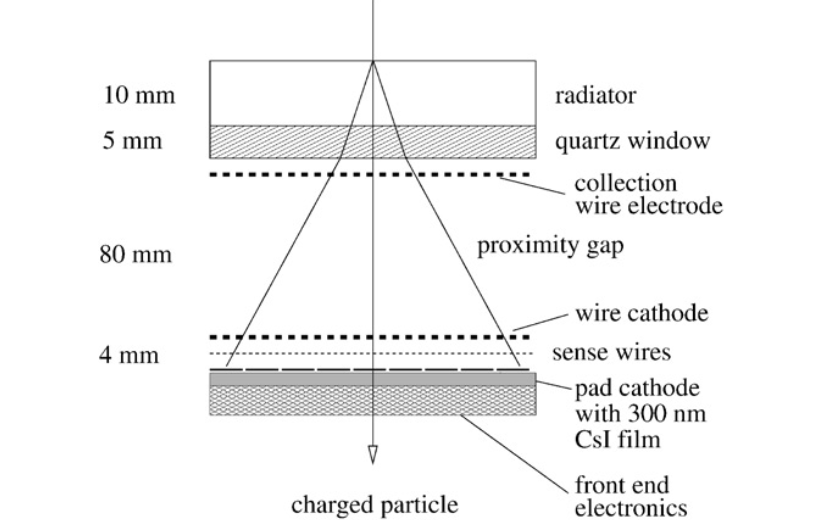
\includegraphics[scale=0.5]{STAR_Detectors/RICH_star_layout}
 		\caption{Δομή του Proximity Focusing RICH}
 		\label{fig3.21}
 	\end{figure}
 	
 	Στον RICH του STAR, ο Cherenkov Radiator είναι $C_6F_{14}$ σε υγρή μορφή και στην συνέχεια υπάρχει ένας κρύσταλλος χαλαζία. 
 	Χρησιμοποιείται η απλούστερη τεχνική Proximity Focusing για την κατεύθυνση των φωτονίων προς την ανιχνευτική περιοχή, κατά την οποία παρεμβάλλεται απλώς ένα στάδιο 80mm κενού χώρου μεταξύ του Radiator και των φωτοανιχνευτών. Ο σκοπός είναι να μεγαλώσει αρκετά η ακτίνα του κύκλου που εν τέλει θα προβληθεί στο επίπεδο του ανιχνευτή και έτσι να έχουε καλύτερη διακριτική ικανότητα.
 	
 	Στο ενδιάμεσο διάκενο ενδέχεται κάποια σωματίδια να ιονίσουν το υλικο και να προκύψουν ελεύθερα ηλεκτρόνια. Προκειμένου να τα απομακρύνουμε από την περιοχή ανίχνευσης έχουμε τοποθετήσει ανόδους κοντά στον Radiator για να τα συλλέγει.
 	Oι συλλογείς των ηλεκτρονίων από ιονισμό είναι τυπικοί Mulitiwire Proportional Chambers (MWPC), με αέριο μεθάνιο, του οποίου οι πρώτες κάθοδοι είναι 100μm σύρματα σε απόσταση 2.2mm από το επίπεδο των ανόδων οι οποίες είναι πάλι σύρματα 20μm που απέχουν μεταξύ τους 4.2mm. 
 	Στην τελική κάθοδο υπάρχουν τοποθετημένα 4 πανελ από ευαίσθητη περιοχή που δίνουν συνολική ενεργό περιοχή 1280$\times 800mm^2$. Στην επιφάνεια της τελικής καθόδου υπάρχει ο φωτομετατροπέας. Ένα λεπτό φιλμ από CsI όπου τα προσπίπτωντα φωτόνια Cherenkov αποβάλλουν ηλεκτρόνια μέσω φωτοηλεκτρικού φαινομένου τα οποία και εν τέλει ανιχνεύουμε ως ρεύμα. Μερικά αποτελέσματα του RICH φαίνονται στις επόμενες Εικόνες.
 	
 	\begin{figure}[h!]
 	    \centering
 	    \begin{minipage}{.5\textwidth}
 	        \centering
 	        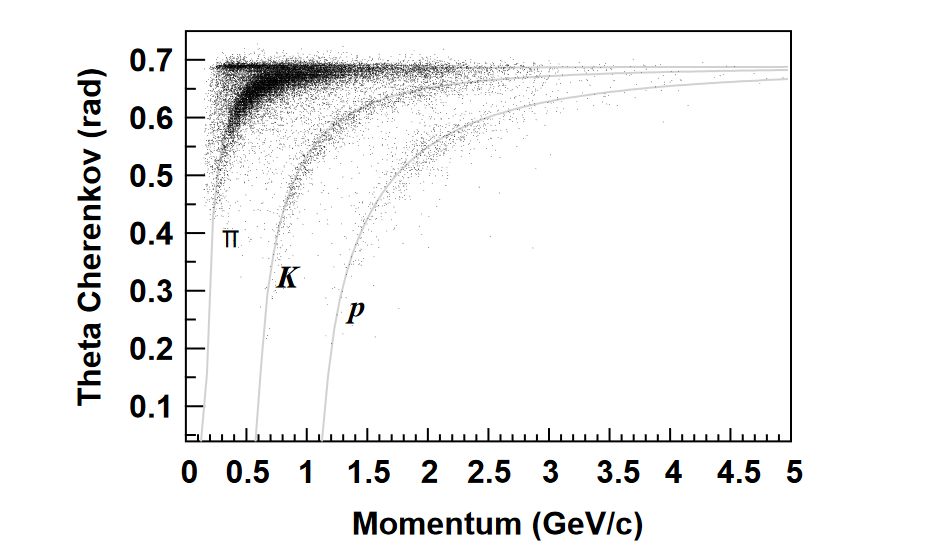
\includegraphics[scale=0.5]{STAR_Detectors/RICH_identif}
 	        \caption{Κατανομή της γωνίας Cherenkov συναρτήσει των μετρήσεων της ορμής που παρέχονται από τον TPC}
 	        \label{fig3.22}
 	    \end{minipage}%
 	    \begin{minipage}{0.5\textwidth}
 	        \centering
 	        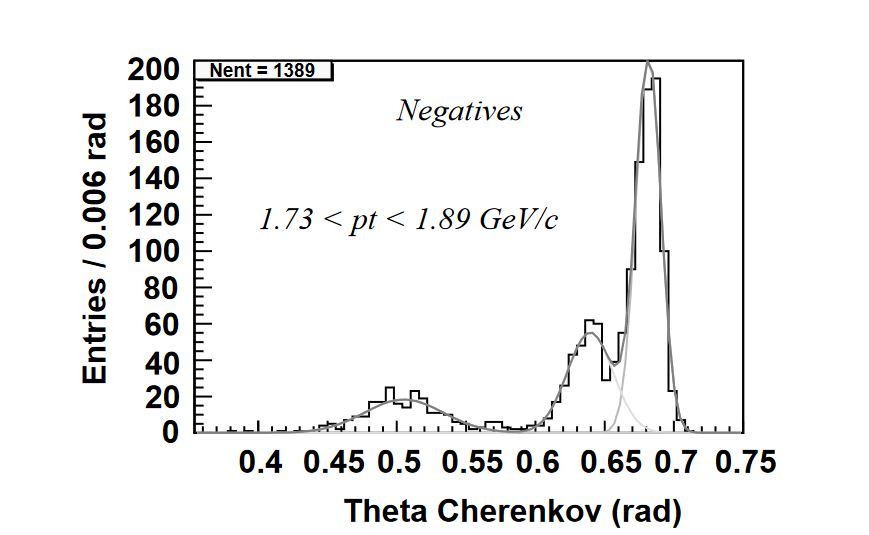
\includegraphics[scale=0.5]{STAR_Detectors/RICH_identif2}
 	        \caption{Ανιχνεύσεις σωματιδίων συναρτήσει της γωνίας Cherenkov για μικρό εύρος ορμών. Οι κορυφές αντιστοιχούν σε πιόνια, καόνια, πρωτόνια.}
 	        \label{fig3.22}
 	    \end{minipage}
 	\end{figure}
 	
 	
 	